	\chapter{粒空间}
\indent

    尽管物理学依旧艰难并且我们依旧困惑依旧有解决不了的问题,但我们已经对之前所能描绘的物理现象有了更清晰的轮廓。所以按道理说,我们应该满意,但是我们还不能止步于此。
    在我们对物理学世界理解的核心中存在一个
\href{http://toyhouse.cc/wiki/index.php/悖论}{悖论}
。那就是为二十世纪遗留给我们的两大物理学珍宝:
\href{http://toyhouse.cc/wiki/index.php/相对论}{相对论}
和
\href{http://toyhouse.cc/wiki/index.php/量子力学}{量子力学}
。
\href{http://toyhouse.cc/wiki/index.php/相对论}{相对论}
推动了宇宙学和
\href{http://toyhouse.cc/wiki/index.php/天体物理学}{天体物理学}
的发展,促进了
\href{http://toyhouse.cc/wiki/index.php/引力波}{引力波}
,
\href{http://toyhouse.cc/wiki/index.php/黑洞}{黑洞}
等很多方面的研究。
\href{http://toyhouse.cc/wiki/index.php/量子力学}{量子力学}
为
\href{http://toyhouse.cc/wiki/index.php/原子物理}{原子物理}
,
\href{http://toyhouse.cc/wiki/index.php/核物理}{核物理}
,基本
\href{http://toyhouse.cc/wiki/index.php/粒子物理}{粒子物理}
,
\href{http://toyhouse.cc/wiki/index.php/凝聚态物理}{凝聚态物理}
和许多方面提供了理论根基。两个理论各自的应用,是我们今天科技的基础,并已经改变了我们的生活方式。但这两个理论至少在现在的形式下一定不都是对的,因为它们之间存在着矛盾。



    一个大学生早晨听了
\href{http://toyhouse.cc/wiki/index.php/相对论}{相对论}
的演讲,下午听了
\href{http://toyhouse.cc/wiki/index.php/量子力学}{量子力学}
的演讲。我们可以谅解他如果他得出了,他的老师是傻子,或者这两个教授已经至少一个世纪都没交流过这样的结论。因为在早晨,演讲中所述的世界是被卷曲的但依旧处处连续的。但在下午,世界就是一个平的空间,处处有量子能级。
    
\href{http://toyhouse.cc/wiki/index.php/悖论}{悖论}
在于这两个理论在实践中都发挥的相当完美。自然正使我们表现的像一个老年法师去调解两个争论不休的男人。已经听完了第一个人的论述,法师说:“你是对的。”,第二个人坚持要陈述观点,法师听完他表述之后说到:“你也是对的。”在隔壁屋里,偶然间听到这谈话的法师的妻子说道:“但他们不可能都是对的啊。”法师沉思了,并且始终纠结于到底“谁说的是对的”。
\footnote[1]
{ 
这里用无比生动形象的
\href{http://toyhouse.cc/wiki/index.php/隐喻}{隐喻}
,写出了相对论与量子力学之间的不可分割的联系以及其极为冲突的内在矛盾。即,相对论认为空间可弯曲但连续,量子力学认为空间是平坦但是量子化。
}

    五湖四海的理论物理学家正费力地尝试去解决这个问题。他们的研究领域叫做“
\href{http://toyhouse.cc/wiki/index.php/圈量子引力论}{圈量子引力论}
”,它的目标是去找一个理论,可以说是一个方程,他可以包含所有的这个世界里可发生的现象,同时它也能解决现在这个精神分裂症般的理论。
    这已经不是第一次物理学家发现他们面对两个高度成功但明显相互矛盾的理论。过去对此的努力使我们很快地认识了我们所在的世界。牛顿靠整合伽利略的
\href{http://toyhouse.cc/wiki/index.php/抛物线}{抛物线}
和开普勒的
\href{http://toyhouse.cc/wiki/index.php/椭圆}{椭圆}
发现了
\href{http://toyhouse.cc/wiki/index.php/万有引力定律}{万有引力定律}
。
\href{http://toyhouse.cc/wiki/index.php/麦克斯韦}{麦克斯韦}
靠整合电学理论和磁场理论发现了电磁场方程组。
\href{http://toyhouse.cc/wiki/index.php/爱因斯坦}{爱因斯坦}
凭借解决明显的电磁学与力学的冲突,提出了
\href{http://toyhouse.cc/wiki/index.php/相对论}{相对论}
。当一名物理学家发现两个成功理论的相矛盾之处会非常高兴,因为这是一个绝佳的机会。但是,我们能依靠思考从这两个理论中学习到的可兼容的世界建立一个概念性的框架吗?
    在这里,学术前沿地带,超越知识的边界,科学变得更加美丽——在幼嫩的想法,直觉和尝试的锻造中变得炙热,耀眼。这也发生在条条道路的兴废中,在热忱中,在想象尚未被想象事物的努力中。
\footnote[2]
{ 
这里“超越知识”愈发说明了,这不仅仅是物理学上的矛盾,而且也是认知科学所需要解决的重大问题,依靠这些问题的解决,我们才得以进一步地探索世界。
}

    二十年前,在这些未知领域有着很浓的迷雾。但是今天曙光已经出现,它已经激起人们的热情和乐观。然而这里不止有一条道路,因此也不能说这个问题已经解决。多重道路产生了争议,但这些争论是健康的:直到迷雾完全散去,有批判和反对的观点就是有利的。尝试去解决这个问题之一的龙头理论的研究方向叫做“
\href{http://toyhouse.cc/wiki/index.php/圈量子引力论}{圈量子引力论}
”。现在这个方向被在各个国家的很多精良的研究小组所信奉
\footnote[3]
{ 
这里为何要将“loop quantum gravity”翻译成“圈量子引力论”,原因如下,loop 是圈,环的意思,而这个理论的主要实质就是整合相对论和量子力学,从而建立自己的理论框架。其提出的微粒空间以及对
\href{http://toyhouse.cc/wiki/index.php/黑洞}{黑洞}
的描述等概念,揭露了宇宙中的某种相似性。而且每个小
\href{http://toyhouse.cc/wiki/index.php/量子}{量子}
在这个理论中也都是相互牵连,像全在一起一样,故翻译成“圈量子引力论”。
}


    
\href{http://toyhouse.cc/wiki/index.php/圈量子引力论}{圈量子引力论}
是一种整合
\href{http://toyhouse.cc/wiki/index.php/广义相对论}{广义相对论}
和
\href{http://toyhouse.cc/wiki/index.php/量子力学}{量子力学}
的尝试。这是一个谨慎的尝试,因为它仅采用了理论已有的假设并适当地改写使之兼容。但它所得的结论却是较为激进的——其深远地颠覆了我们观察现实结构的方式。
    这个想法是简单的。
\href{http://toyhouse.cc/wiki/index.php/广义相对论}{广义相对论}
已经告诉我们,空间不是一个惰性的长方盒,而是一种动态的东西:一种包含我们在内的,巨大的可移动的,可以被压缩,卷曲的蜗牛壳。另一方面,
\href{http://toyhouse.cc/wiki/index.php/量子力学}{量子力学}
已经告诉我们一切场都是由
\href{http://toyhouse.cc/wiki/index.php/量子}{量子}
组成的,并且有良好的颗粒状的结构。紧随而来的结论就是,物理空间也是由量子组成。


    
\href{http://toyhouse.cc/wiki/index.php/圈量子引力论}{圈量子引力论}
的中心结论确实指出空间不是连续的,而且其不是无限可分的而是由微小粒子组成或者说是“原子空间”组成。它们是极小的:比最小的
\href{http://toyhouse.cc/wiki/index.php/原子核}{原子核}
的一亿亿分之一还要小。这个理论描述了这些“原子空间”在数学上的形式,并提供了决定它们演化方式的方程。这些方程被称为“圈”,或者环,因为他们相互联系,组成了网状结构。这种网状结构像精细编织的巨大锁子匣一样,编织出了空间材质。
\footnote[4]
{ 
按照史瓦西半径公式和康普顿波长公式,使史瓦西半径等于康普顿波长时,它们的长度即为普朗克长度,大约1.6e-35(同时质量等于普朗克质量)。在该长度尺度下,经典的引力理论包括相对论都会失效。因为小于该尺度的任何有质量物质不确定性域小于史瓦西半径,并因此坍缩而失去意义。这意味着在这个特别的尺度下引力场具有完全不同以往认知的结构。自然的,圈量子引力的原子空间必定会关注这个特别尺度,而它们的大小和普朗克长度相近。
}

    那这些空间量子在哪呢?哪也不在。它们不存在于空间,因为它们本身即空间。空间靠连接这些独立的引力量子而被创造。又一次,世界看起来,相比于是关于物体的,更像是关于交互关系的。
    但是这是该理论的第二个结论,也是最极端的结论。正如连续的空间包含着物体的想法不存在一样,所以基本的原始的与物体无关的绝对流逝的时间亦消失了。描述空间颗粒和物质的方程不再含有时间变量。但这不意味着任何事物都是静止的和不变的。正相反,这意味着改变是无处不在的——但是基本过程不能够被排列为一个普通的“极小瞬间”的序列。在非常小的粒空间尺度上,自然的舞蹈不能每一个节拍都依照管弦乐团指挥官手中指挥棒的节奏:因为其每个过程的舞蹈都独立于其旁边的舞者有他自己的节奏。时光流逝是世界的内在规律,它诞生于世界中的两个量子事件之间,量子事件包含着世界并且它们自己就是时间的来源。
    在这个理论描述下的世界因此变得和我们所熟悉的世界更加遥远。这里不再有空间包含世界,也不再有时间中发生事件。这里只有基本进程。在进程中,空间和物质量子不断相互影响。我们身边连续的空间和时间的幻象其实是我们依稀看到的模糊不清的对集群的基础过程的混乱的视野。就像风平浪静的阿尔卑斯湖实际上包含无数快速舞蹈的微小
\href{http://toyhouse.cc/wiki/index.php/水分子}{水分子}
。
    通过超强的放大镜,用考察极端的特写镜头。在如下的图片中展示了空间的颗粒结构。

\begin{figure}[htbp]
\begin{minipage}[t]{0.3\linewidth}
\centering
\bc
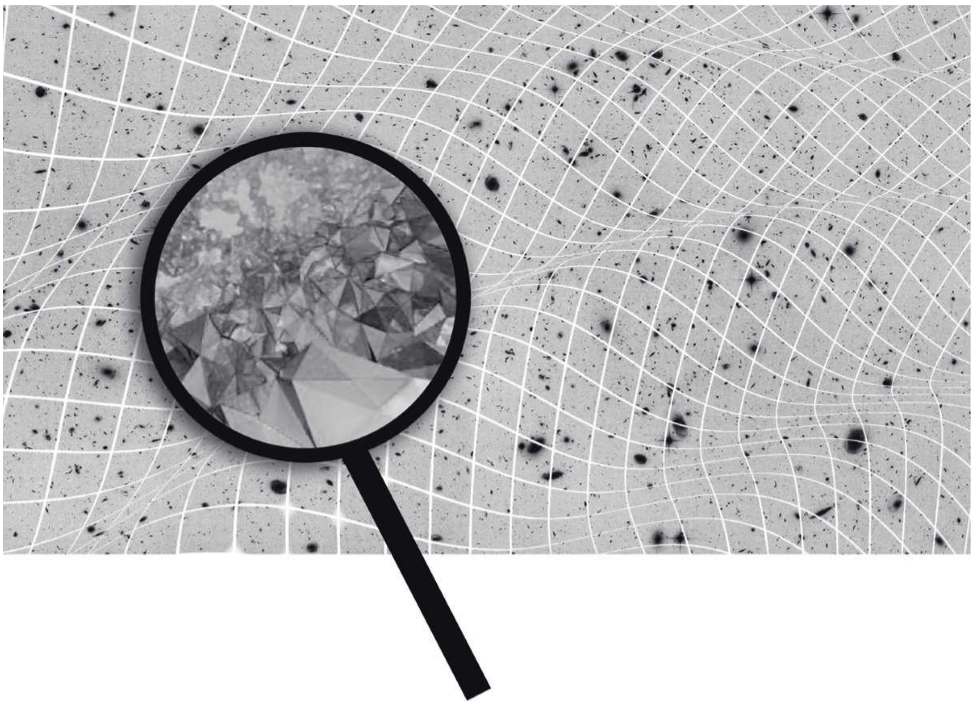
\includegraphics[width=3\textwidth]{img/51.png}\\[12pt]
\ec
\caption{我们在第三章已经见到这幅图像的背景了。没错,就是那张哈勃望远镜拍摄的宇宙图景基础加上表示弯曲空间的辅助线的图片。按照原文“通过甚强的放大镜,用考察极端的特写镜头”,我们便看到了放大镜中间的图像,也就是宇宙在极小尺度下的图像。对于化学或者材料稍微熟悉的人,规整的起伏和一些排列在一起的晶胞还是非常相像的;让这个比喻再通俗一点,就好像非常多盐的颗粒平整地撒在桌面上。在图像中,这些“晶胞”或者“颗粒”不是紧致的堆在背景当中,在近处它们聚在一起,但稍远处可以看到它们集束成多条纤维。通过这个细节,文章也展示了原文中不够形象的部分,比如,“‘环’组成了网状结构”和“像精细编织的巨大锁子匣一样,编织出了空间材质”。}
\label{fig:side:a}
\end{minipage}

\end{figure} 


    有可能实验验证这个理论吗?我们思考着尝试着,但是还没有实验的验证。无论如何,有一些不同的尝试。
    这些尝试中的一支派生出了
\href{http://toyhouse.cc/wiki/index.php/黑洞}{黑洞}
的研究。在天空中我们已经可以观察坍缩恒星形成的
\href{http://toyhouse.cc/wiki/index.php/黑洞}{黑洞}
。这些
\href{http://toyhouse.cc/wiki/index.php/恒星}{恒星}
被自身质量压碎,向自身塌陷,以及从我们的视野中消失。但是它去哪了?如果
\href{http://toyhouse.cc/wiki/index.php/圈量子引力论}{圈量子引力论}
是正确的,物质不可能真正探索到一个无穷的点上,因为不存在只有有限大小的宇宙块。在自身的重量下坍缩,物质一定会变得更加稠密,直到某个时刻,在这个时刻
\href{http://toyhouse.cc/wiki/index.php/量子力学}{量子力学}
一定会产生反作用的
\href{http://toyhouse.cc/wiki/index.php/平衡力}{平衡力}
。
    在假设的恒星生命的最后阶段就是人们所知的“普朗克星”。在这一阶段中时空量子涨落平衡了物质自身重量。如果太阳停止燃烧,形成一个
\href{http://toyhouse.cc/wiki/index.php/黑洞}{黑洞}
,黑洞直径将会有约一点五公里。在这个黑洞中心,太阳的物质将会继续坍缩,最终成为
\href{http://toyhouse.cc/wiki/index.php/普朗克星}{普朗克星}
。它的尺度就和那些原子的尺度差不多。太阳全部的物质被压缩进一个原子的空间:一个普朗克星应该是由这样极端状态的物质构成的。
    普朗克星不是不稳定的:一旦压缩到极限,它就会反弹,开始重新膨胀。这会导致一次黑洞爆炸。就像一个坐在黑洞中普朗克星上的假设观察者,这个过程将会是一个发生得极快的反弹。但是对于这个观察者,那些在黑洞外面的人时间不会以同样的速度流逝。同样的道理,在山上时间会比在海平面流逝得更快。除非她以外,因为极端条件,时间片段的差别是巨大的,并且对于恒星上观察者极快的反弹,对外面的人来说显得是在很长一段时间发生的事。这就是为什么我们观察黑洞总是在相当长时间中保持不变:黑洞是以看起来极端缓慢的动作正在反弹。
    有可能在第一批宇宙黑洞形成的大熔炉中,黑洞中的一部分正在爆炸。我们如果是正确的,就很可能观测到它们爆炸所激发出的,以来自太空高能宇宙射线形式的信号。这也允许我们观测和测量量子引力主导现象的直接效应。这是一个大胆的想法——它有可能失效,比如可能在原始宇宙没有形成足够多的黑洞,能让我们今天来探测它们的爆炸。但是这个信号的探索研究已经展开。我们将来会看到结果。
    这个理论的另一个结论,也是最壮观的结论之一,关系到宇宙的起源。我们知道怎样重建我们行星的历史,直到最初的,它还很小的时期。但是在那之前呢?对的,圈理论的方程允许我们回溯得更远,重建它的历史。
    我们可以发现当宇宙还极度压缩的时候,量子理论产生了斥力,导致了巨大的爆炸,“大爆炸”或者事实上是“大反弹”。事实上,我们的世界可能诞生自从,反弹之前的一个宇宙。这个宇宙在自身重力下坍缩到一个极小空间,正要重新膨胀,从而成为我们观测到的,身边正在膨胀的宇宙。
    在这个反弹的瞬间,宇宙坍缩进一个坚果壳内,是真正的量子引力的领域:时间和空间同时消失了,世界被溶化成一团集群的概率云。然而我们的方程依然能描述这个概率云。第五堂课的最终图景被转换成下图:

\begin{figure}[htbp]
\begin{minipage}[t]{0.3\linewidth}
\centering
\bc
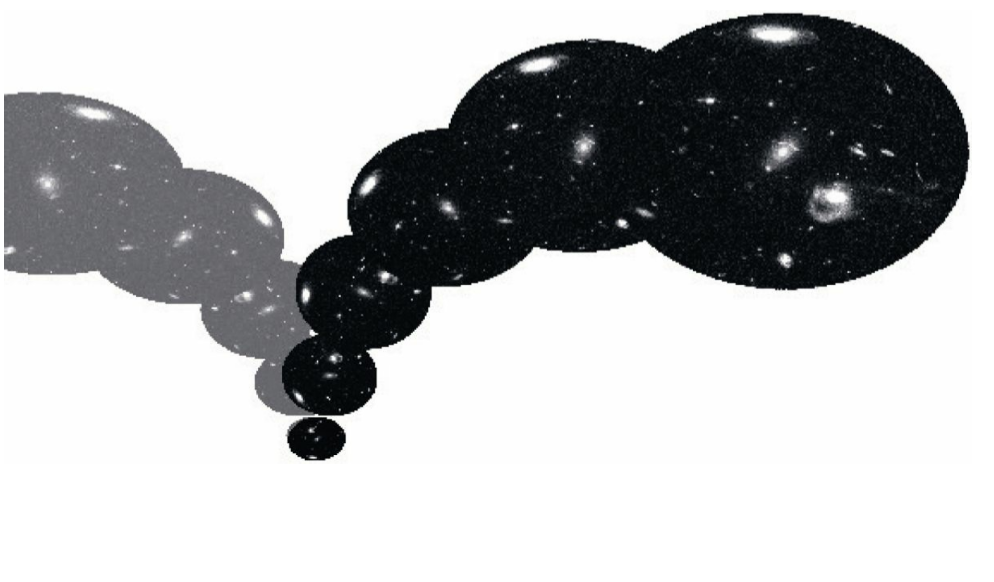
\includegraphics[width=3\textwidth]{img/52.png}\\[12pt]
\ec
\caption{可能在很多别的科普书中,我们看到过类似“实体”的右半支图像被用于形象描述我们的宇宙膨胀状态。在这里也概莫能外,事实上我们的宇宙也确实在加速膨胀。相对“虚”的,或者说有些透明的左半支则是一个相反的过程,宇宙的收缩状态。“虚”或者透明则是因为这是上一个宇宙对于现在的我们是不可观测的,目前我们没有任何手段能够预言并检测这个宇宙在反弹中的诞生之前的宇宙的任何有关讯息。}
\label{fig:side:a}
\end{minipage}

\end{figure} 

    我们的宇宙可能诞生自先前阶段的反弹,并经过一个既没有空间也没有时间的中间阶段。
    物理打开了一扇窗,从中我们可以看得很远,我们所见将会一直震惊我们。我们意识到,自身充满偏见,自身对世界的直觉图景也是偏颇的,狭隘的,也是不恰当的。世界不是平坦的,也不是静止的。世界将在我们眼前继续变化,我们逐渐能够将它看得更广阔,看得更清晰。如果我们尝试整理我们在二十世纪关于物理世界的所学,线索将会指向和我们对物质,空间和时间的直觉理解有深刻差异的事物上。圈量子引力论是一个企图破译这些线索的尝试,也是看向更远的一点距离的尝试。
\footnote[5]
{ 
作者本人也是圈量子引力论的提出者之一。
}


\noindent
